%%%% Document type  %%%%
\documentclass[preprint,12pt,fleqn]{article}
 \usepackage{ragged2e}
\usepackage{authblk}  % Package for author affiliations
% \usepackage{nopageno} % no page numbers
\usepackage{placeins} % \FloatBarrier

\usepackage[most]{tcolorbox}
\newtcolorbox[auto counter,number within=chapter]{definition}[1][]{
  enhanced,
  breakable,
  fonttitle=\scshape,
  title={Definition \thetcbcounter},
  #1
}

%%%% Document structure %%%%
%\usepackage{geometry}
\usepackage[verbose=true,letterpaper]{geometry}
\geometry{
%    a4paper,
%    left=30mm,
%    right=30mm,
%    top=30mm,
%    bottom=30mm,
    textheight=9in,
    textwidth=6in,
    top=1in,
    headheight=12pt,
    headsep=25pt,
    footskip=30pt,
   % phone  
   %a5paper,
   %width=120mm,
  %height=180mm,
}

\usepackage{lineno} % used along with \linenumbers after begin document. 
\usepackage{setspace} 
% \setstretch{1.4}
\makeatletter % The following lines get rid of footer stating pre-preint to elsevier.
\def\ps@pprintTitle{%
\let\@oddhead\@empty
\let\@evenhead\@empty
\def\@oddfoot{}%
\let\@evenfoot\@oddfoot}
\makeatother
\graphicspath{ {../images/} }
\usepackage{pgf} % calculate cohort stats percentage

%%%% Bibliography   %%%%
\usepackage{natbib}
\setcitestyle{numbers,sort&compress}
\setcitestyle{sort&compress}
\usepackage{hypernat} 
    
%%%% Aesthetics     %%%%
\usepackage{microtype}
% \RequirePackage{times} % Font
\usepackage{ccaption}
\usepackage{siunitx}
\usepackage[T1]{fontenc}
\usepackage[utf8]{inputenc}
\usepackage{nameref}% this allows a reference be named, to print unnumbered references by their section name (used here for linking to Supplemental text in this case).

%%%% Paragraph Formatting %%%
\setlength{\parindent}{0pt}
\setlength{\parskip}{6pt plus 2pt minus 1pt}

%%%% Supplemental labels%%%%
%Define command to start a supplemental section
%set the supplemental letter used for figures (e.g. Figure E1)
\newcommand{\beginsupplement}{%
        \setcounter{table}{0}
        \renewcommand{\thetable}{S\arabic{table}}%
        \setcounter{figure}{0}
        \renewcommand{\thefigure}{S\arabic{figure}}%
         }

%%%% Building tables%%%%
\usepackage{booktabs} % required for tables
\usepackage{rotating,tabularx} 
\newcolumntype{Z}{ >{\centering\arraybackslash}X } % defining table content layout per box
\usepackage{ltablex} % allow page break between lines in tabularx
% \usepackage{caption} \captionsetup{font=normalsize} % to set the caption size as normal even when table is tiny.
\usepackage{multirow}
\usepackage{pdflscape}

%%%% Colors %%%%
\usepackage{xcolor} 
\definecolor{natureblue}{RGB}{5,110,210}
    \usepackage[colorlinks]{hyperref} 
\AtBeginDocument{%this allows colours to chage from the defined elsearticle template.
\hypersetup{
    	colorlinks=true,
        linkcolor={natureblue},
    	citecolor={natureblue},
        filecolor=blue!50!black,
        urlcolor=cyan,
    	}}

\definecolor{kispiblack}{HTML}{333333}
\definecolor{kispidarkblue}{HTML}{023047}
\definecolor{kispidarkgreen}{HTML}{006666}
\definecolor{kispired}{HTML}{C70000}
\definecolor{kispilink}{HTML}{007DB8}%219EBC
% \color{kispi_black} %default
\definecolor{kispiblue}{HTML}{701A57}
% City sunset: https://www.color-hex.com/color-palette/40131
\definecolor{colorSUNSET1}{HTML}{eeaf61}
\definecolor{colorSUNSET2}{HTML}{fb9062}
\definecolor{colorSUNSET3}{HTML}{ee5d6c}
\definecolor{colorSUNSET4}{HTML}{ce4993}
\definecolor{colorSUNSET5}{HTML}{6a0d83}
\definecolor{natureblue}{RGB}{5,110,210}    
\usepackage{dirtree}  % Load the dirtree package


% command to use these colors and formatting; xspace for correct spacing including with punctuation marks.
\usepackage{xspace}
\newcommand{\variablesdarkgreen}[1]{\textbf{\textcolor{kispidarkgreen}{#1}}\xspace}

%%%% Fancy stuff %%%%
%\usepackage{fancyhdr}
%\pagestyle{fancy}
%\lhead{My Name}
%\chead{}
%\rhead{\thepage}
%\cfoot{} % get rid of the page number 
%\renewcommand{\headrulewidth}{0pt}
%\renewcommand{\footrulewidth}{0pt}
 
 
%\usepackage{fancyhdr}
%\usepackage{lastpage}
%\pagestyle{fancy}
%\fancyhf{}
%\rfoot{\thepage}
%\cfoot{} % get rid of the page number 
%\renewcommand{\headrulewidth}{0pt}
%\renewcommand{\footrulewidth}{0pt}

 
\usepackage{tocloft}  % Customizing the Table of Contents
\setcounter{tocdepth}{2}


%%%% Include code %%%%
% \usepackage{verbatim}

\usepackage{listings}
\lstset{
    basicstyle=\ttfamily\small,
    breaklines=true,
    postbreak=\mbox{\textcolor{red}{$\hookrightarrow$}\space}, % 
    breakatwhitespace=false,
    % frame=single,
    showstringspaces=TRUE, % Don't show spaces in strings as special characters
    tabsize=2, 
    language=sh 
}

\usepackage{fontspec}
% \setmainfont{IBM Plex Sans}
% \setmonofont{IBM Plex Mono}
% \usepackage{unicode-math}
% \setmathfont{IBM Plex Math}

%\renewcommand{\rmdefault}{ptm}
%\renewcommand{\sfdefault}{phv}


% {{\ttfamily \hyphenchar\the\font=`\-} % set hyphenation for texttt blocks









% nips 2017 settings


\usepackage[printonlyused,withpage,nohyperlinks]{acronym}

\begin{document}
\title{Supplemental - PanelAppRex aggregates disease gene panels and facilitates sophisticated search}	

% in your preamble, before \author:
\newcommand{\QUANT}{1}
\newcommand{\GHI}{2}
\newcommand{\LEEDS}{3}
\newcommand{\IPSNEO}{4}

\author[\QUANT]{Quant Group} 
\author[\GHI]{Simon Boutry}% \textsuperscript{†}}
\author[\GHI]{Ali Saadat}% \textsuperscript{†}} \textsuperscript{†}}
\author[\LEEDS]{Sinisa Savic}% orcid.org/0000-0001-7910-0554
\author[\IPSNEO]{Luregn J. Schlapbach}
\author[\GHI]{Jacques Fellay}
\author[\IPSNEO]{Dylan Lawless \thanks{Addresses for correspondence: \href{mailto:Dylan.Lawless@kispi.uzh.ch}{Dylan.Lawless@kispi.uzh.ch}}
}

%\author[\KISPIIMM]{Maarja Soomann}% \textsuperscript{†}} \textsuperscript{†}}
%\author[\KISPIIMM]{Johannes Trück}
\affil[\QUANT]{The quantitative omic epidemiology group.} 
\affil[\GHI]{Global Health Institute, School of Life Sciences, École Polytechnique Fédérale de Lausanne, Switzerland.}
\affil[\LEEDS]{Leeds Institute of Rheumatic and Musculoskeletal Medicine, University of Leeds, Leeds, UK.}
\affil[\IPSNEO]{Department of Intensive Care and Neonatology, University Children's Hospital Zurich, University of Zurich, Zurich, Switzerland.}

\maketitle
\justify

%\\\\\\\\\\\\\\\\\\\\\\\\\\\\
\clearpage
\beginsupplement
\section*{Supplemental} \label{Supplemental_text}


\begin{table}[htbp]
\caption{\textbf{Summary of case study queries and PanelAppRex results.} 
``Subjective best panels'' are those reasonably preferable to the clinical query and unlikely to be excluded by users. In the benchmark scenario, broad or less relevant panels (e.g. ``COVID-19 research'') might be deprioritised in favour of more clinically aligned options such as ``Fetal anomalies'', or ``Paediatric disorders''. Summarised in \textbf{Figure 1}.
*Case study 5 had five individual cases and patient information was significantly longer than other studies. Therefore, we used OpenAI model o3-mini to converted it to a standardised keyword query automatically, thereby removing our subjective bias and aligning with the other queries.
}
\label{tab:benchmark}
\centering
\resizebox{\textwidth}{!}{
\begin{tabular}{|
    p{1cm}|
    p{4cm}|
    p{4cm}|
    p{1.4cm}|
    p{1.3cm}|
    p{1.3cm}|
    p{1.3cm}|
    p{1.3cm}|
    p{1.3cm}|
    p{5cm}|}
\hline
\textbf{Case study}	(\textbf{Ref})	 & 	\textbf{Source title}	 & 	\textbf{Query}	 & 	\textbf{Causal gene}	 & 	\textbf{Result panels}	 & 	\textbf{Subjective best panels}	 & 	\textbf{Panels with causal gene}	 & 	\textbf{Subjective relevance ratio}	 & 	\textbf{Causal gene in all results}	 & 	\textbf{Result ID, panelName, geneCount} \\
\hline																			
1	\cite{arruda_genetic_2015}	 & 	Genetic Analysis As a Practical Tool to Diagnose Hereditary Angioedema with Normal C1 Inhibitor: A Case Report	 & 	SERPING1 Factor XII edema	 & 	F12	 & 	3	 & 	1	 & 	3	 & 	0.3	 & 	1	 & 	64 COVID-19 research 695; 192 Primary immunodeficiency or monogenic inflammatory bowel disease 572; 311 Research panel - Severe Paediatric Disorders 2691 \\
\hline																			
2	\cite{mcaleer_severe_2015}	 & 	Severe dermatitis, multiple allergies, and metabolic wasting syndrome caused by a novel mutation in the N-terminal plakin domain of desmoplakin	 & 	SAM syndrome DSG1 dermatitis metabolic wasting	 & 	DSP	 & 	3	 & 	3	 & 	3	 & 	1	 & 	1	 & 	205 Fetal anomalies 2185; 210 DDG2P 2422; 211 Paediatric disorders 3903 \\
\hline																			
3	\cite{verhoeven_hematopoietic_2022}	 & 	Hematopoietic stem cell transplantation in a patient with proteasome-associated autoinflammatory syndrome (PRAAS)	 & 	resistant cutaneous vasculitis SH2D1A	 & 	PSMB4	 & 	3	 & 	1	 & 	2	 & 	0.3	 & 	0.7	 & 	64 COVID-19 research 695; 192 Primary immunodeficiency or monogenic inflammatory bowel disease 572; 311 Research panel - Severe Paediatric Disorders 2691 \\
\hline																			
4	\cite{magerus-chatinet_autoimmune_2013}	 & 	Autoimmune lymphoproliferative syndrome caused by a homozygous null FAS ligand (FASLG) mutation	 & 	Autoimmune lymphoproliferative syndrome ALPS lymphoproliferation hypergammaglobulinemia autoimmune cytopenia	 & 	FASLG	 & 	2	 & 	1	 & 	2	 & 	0.5	 & 	1	 & 	64 COVID-19 research 695; 192 Primary immunodeficiency or monogenic inflammatory bowel disease 572 \\
\hline																			
5*	\cite{sharfe_fatal_2014}	 & 	Fatal combined immunodeficiency associated with heterozygous mutation in STAT1	 & 	primary immunodeficiency recurrent pneumonia chronic diarrhea oral thrush bronchiectasis lymphadenopathy hepatosplenomegaly autoimmune hepatitis Addison	 & 	STAT1	 & 	1	 & 	1	 & 	1	 & 	1	 & 	1	 & 	192 Primary immunodeficiency or monogenic inflammatory bowel disease 572 \\
\hline
\end{tabular}
}
\end{table}





\begin{figure}[ht]
    \centering
    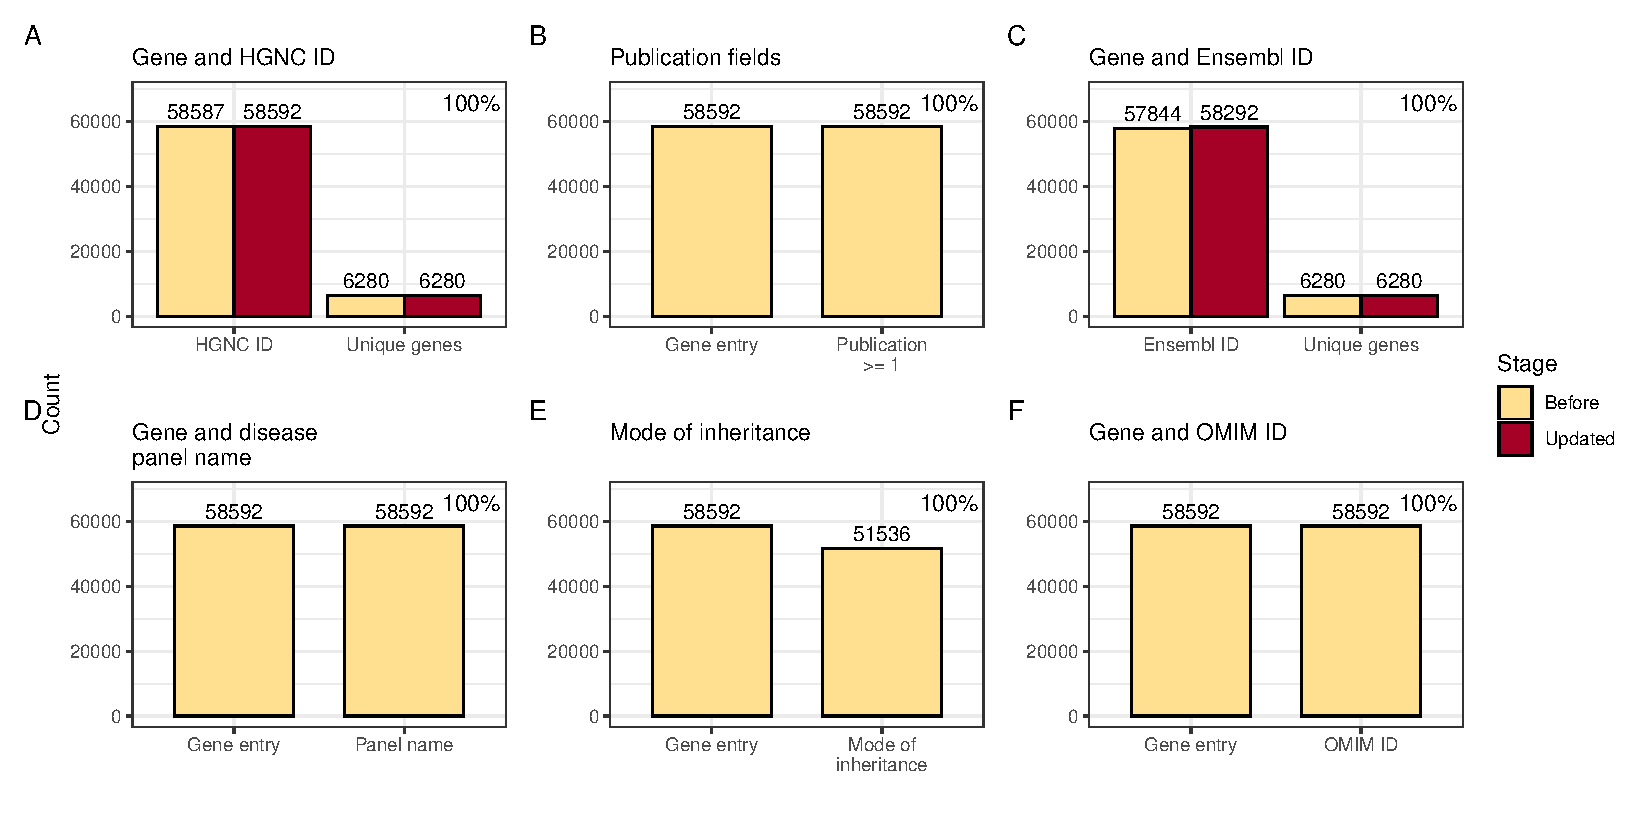
\includegraphics[width=0.99\textwidth]{validation_counts.pdf}
\caption{\textbf{Validation and recovery of core annotation fields in the PanelAppRex dataset.}
(A) Unique genes and HGNC IDs before and after retrieving missing HGNC entries via Ensembl.
(B) Availability of publication annotations for genes.
(C) Unique genes and Ensembl gene IDs before and after biomart-based recovery of missing Ensembl IDs.
(D) Gene entries with associated disease panel names.
(E) Gene entries with annotated \ac{moi}.
(F) Gene entries linked to an OMIM gene ID.
Each bar shows the count of entries with non-missing values for the respective field. Updated fields (HGNC and Ensembl ID) reflect values recovered via external lookup using HGNC symbols. Percentage shows the complete recovery of coverage across features.
}
    \label{fig:validation}
\end{figure}




















\begin{figure}[ht]
    \centering
    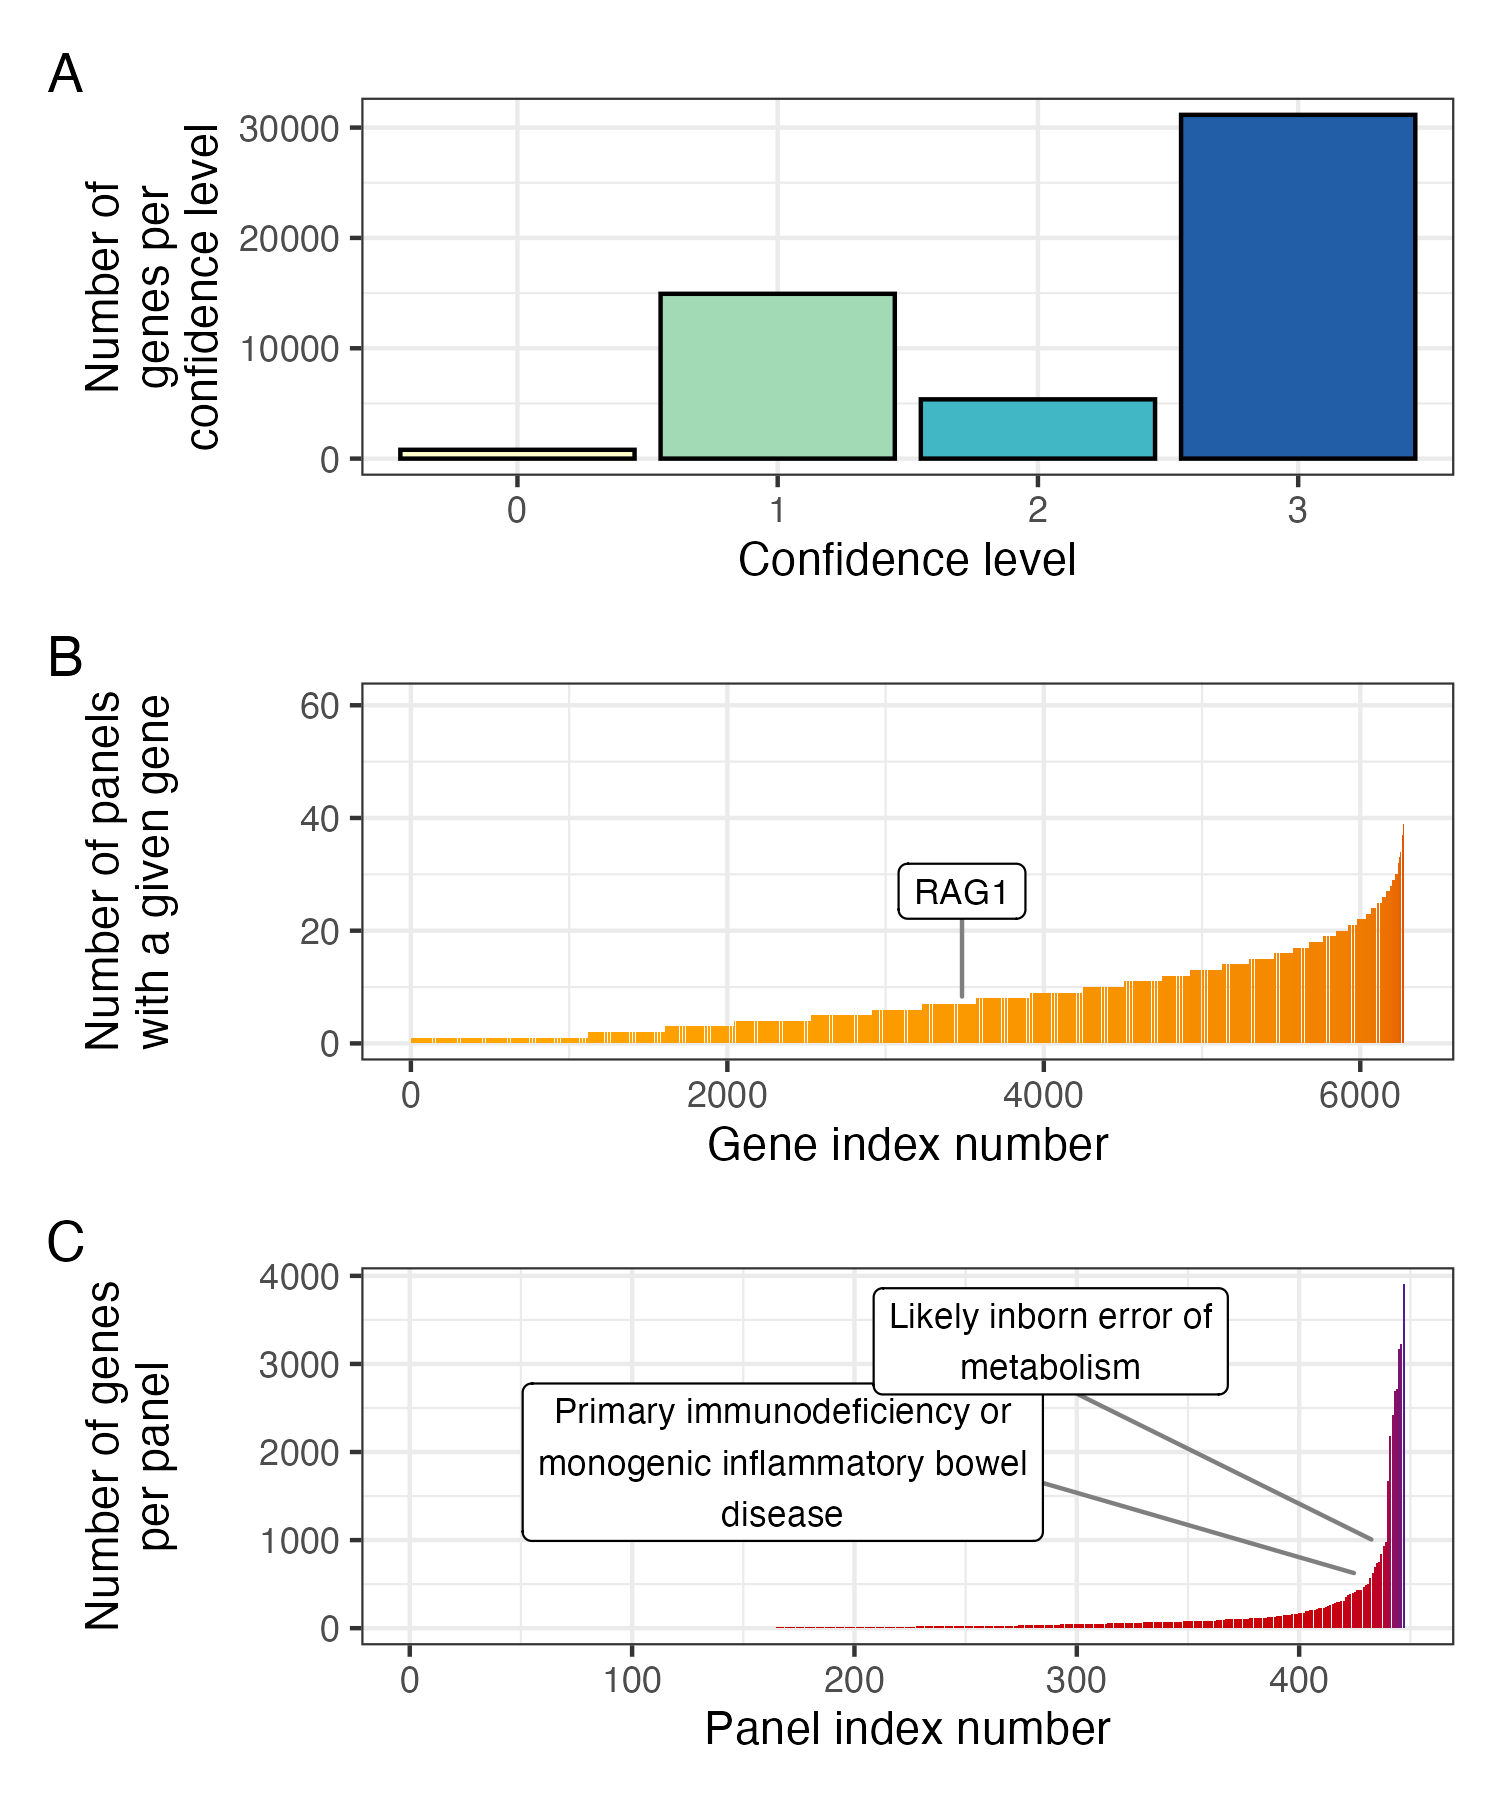
\includegraphics[width=0.75\textwidth]{plot_patch2_annotated_example.png}    
\caption{\textbf{Summary of gene confidence levels, reuse across panels, and panel sizes in the PanelAppRex dataset.}
(A) Number of genes per confidence level. 
(B) Number of panels in which each gene is included, with the example gene \textit{RAG1} highlighted to demonstrate that it is present in 7 panels. 
(C) Number of genes per panel, with two representative panels annotated: panel ID 398 (\ac{pid}/\ac{iei}) and panel ID 1220 (\ac{iem}).
}
    \label{fig:summary_stats}
\end{figure}


\begin{figure}[ht]
    \centering
    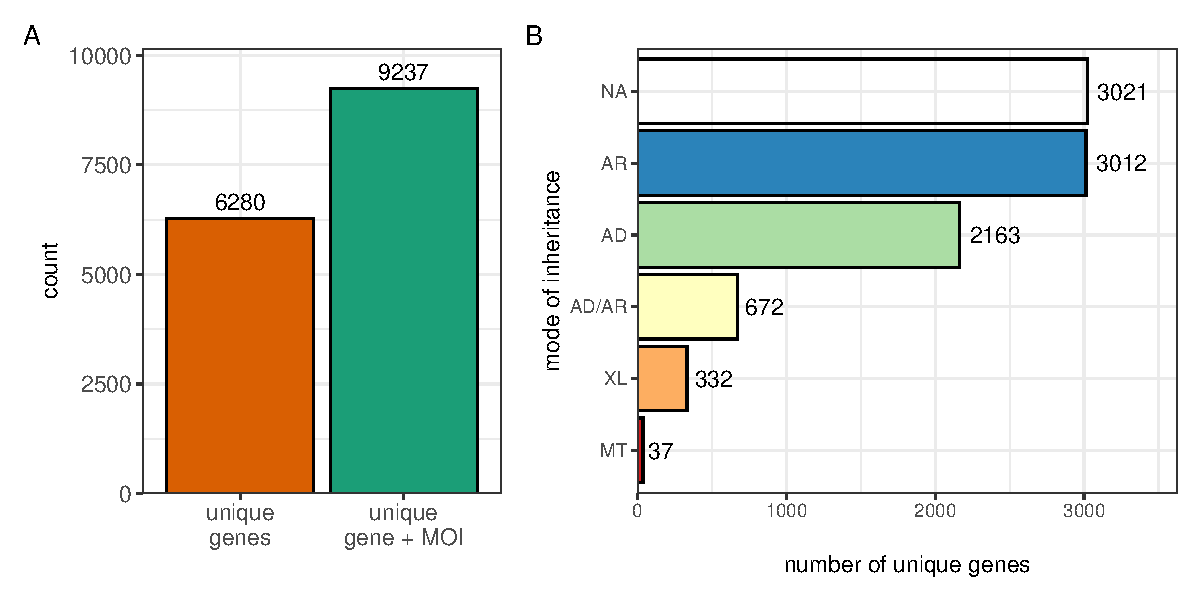
\includegraphics[width=0.99\textwidth]{plot_patch_uniq_gene_moi_summary.pdf}
\caption{\textbf{Summary of mode of inheritance annotations in the PanelAppRex dataset.}
(A) Counts of unique genes annotated with each \ac{moi}, based on non-redundant gene-\ac{moi} combinations.
(B) Total number of unique genes and total number of gene-\ac{moi} combinations in the harmonised PanelAppRex dataset.
}
    \label{fig:uniq_gene_moi}
\end{figure}

\begin{figure}[ht]
    \centering
    
\includegraphics[width=0.99\textwidth]{panelapprex_logo_v2_16x9.png}
\caption{\textbf{(logo)} PanelAppRex reigns over genomic complexity.
}
    \label{fig:uniq_gene_moi}
\end{figure}

\FloatBarrier
\clearpage
\bibliographystyle{unsrtnat}
\bibliography{references.bib}


\end{document}
